\documentclass[11pt]{article}
\usepackage[margin=1in]{geometry}
\usepackage{amsmath,amssymb,booktabs,graphicx,setspace,caption,hyperref}
\usepackage[T1]{fontenc}
\usepackage{mathpazo}
\setlength{\parindent}{0pt}
\setlength{\parskip}{0.6em}
\captionsetup{font=small,skip=6pt}
\title{Panel MS-AR(1): common intercept and linear trend\\[0.4em]\large 1985 through the end of the sample, excluding the US, Germany, Japan, and China}
\author{}
\date{}
\begin{document}
\maketitle
\section{Model}
Seasonally adjusted real GDP per worker, 2026-09-17 vintage, 1985-Q1 through 2026-Q2. United States, Germany, and Japan are excluded. China is not in this vintage.
\begin{align}
y_{it} &= a + g\, t + z_{it}, \\
s_{i,t+1} &\sim \Pi(\,\cdot\mid s_{it}), \\
z_{i,t+1} &= \bigl(1-\rho(s_{i,t+1})\bigr)\mu(s_{i,t+1}) + \rho(s_{i,t+1})\, z_{it} + \sigma(s_{i,t+1})\,\varepsilon_{it}.
\end{align}
The regime $s_{it}$ is the one that produced $z_{it}$. $\varepsilon_{it}$ is the innovation. $g$ is the within-country slope, so a country that enters later does not shift $g$ through its level. $a$ is then set so that $z_{it}=y_{it}-a-gt$ has mean zero. Three regimes. The MS-AR imposes $E[z]=0$. $\sigma$ and $\rho$ switch, with $|\rho|<0.99$. Standard errors are delta-method from a numerical Hessian of the cycle parameters. $a$ and $g$ have none.
\clearpage
\section{Common intercept and linear trend, 1985 through the end of the sample, ex US, Germany, Japan, China}
2026-09-17 SA panel, 1985-Q1 through 2026-Q2, excluding the US, Germany, and Japan. $y_{it}=a+gt+z_{it}$, $g$ the within-country slope, $E[z]=0$. 71 countries, 7893 observations, 1985-Q1--2026-Q2. Fitted countries: 71. Observations: 7893. Log-likelihood: 20160.06.
The within-country slope is $g=0.0164$ and the intercept that zeros the pooled mean of $z$ is $a=-5.3569$ (no standard errors). $a$ is the intercept at the first date in the estimation sample. $z_{it}=y_{it}-a-gt$ is the cycle in the figure. Its average within-country slope is zero. The MS-AR is the law of $z$, with $E[z]=0$.
\begin{table}[h]
\centering
\caption{Regime AR(1), transition matrix, and ergodic $\pi$. Columns are regimes.}
\begin{tabular}{lccc}
\toprule
 & (0) & (1) & (2) \\
\midrule
$\mu$ & -0.7737 & -0.7471 & 1.1467 \\
 & (0.0749) & (0.0374) & (0.0140) \\ \addlinespace
$\sigma$ & 0.0733 & 0.0159 & 0.0098 \\
 & (0.0021) & (0.0003) & (0.0002) \\ \addlinespace
$\rho$ & 0.9900 & 0.9900 & 0.9900 \\
 & (0.0000) & (0.0000) & (0.0000) \\ \addlinespace
$\Pi_{0\cdot}$ & 0.7223 & 0.2000 & 0.0777 \\
 & (0.0255) & (0.0221) & (0.0103) \\ \addlinespace
$\Pi_{1\cdot}$ & 0.0610 & 0.9385 & 0.0005 \\
 & (0.0059) & (0.0058) & (0.0012) \\ \addlinespace
$\Pi_{2\cdot}$ & 0.0284 & 0.0000 & 0.9716 \\
 & (0.0033) & (0.0004) & (0.0033) \\ \addlinespace
$\pi$ & 0.1419 & 0.4616 & 0.3965 \\
 & (0.0107) & (0.0154) & (0.0110) \\ \addlinespace
\bottomrule
\end{tabular}
\end{table}
\begin{figure}[h]
\centering
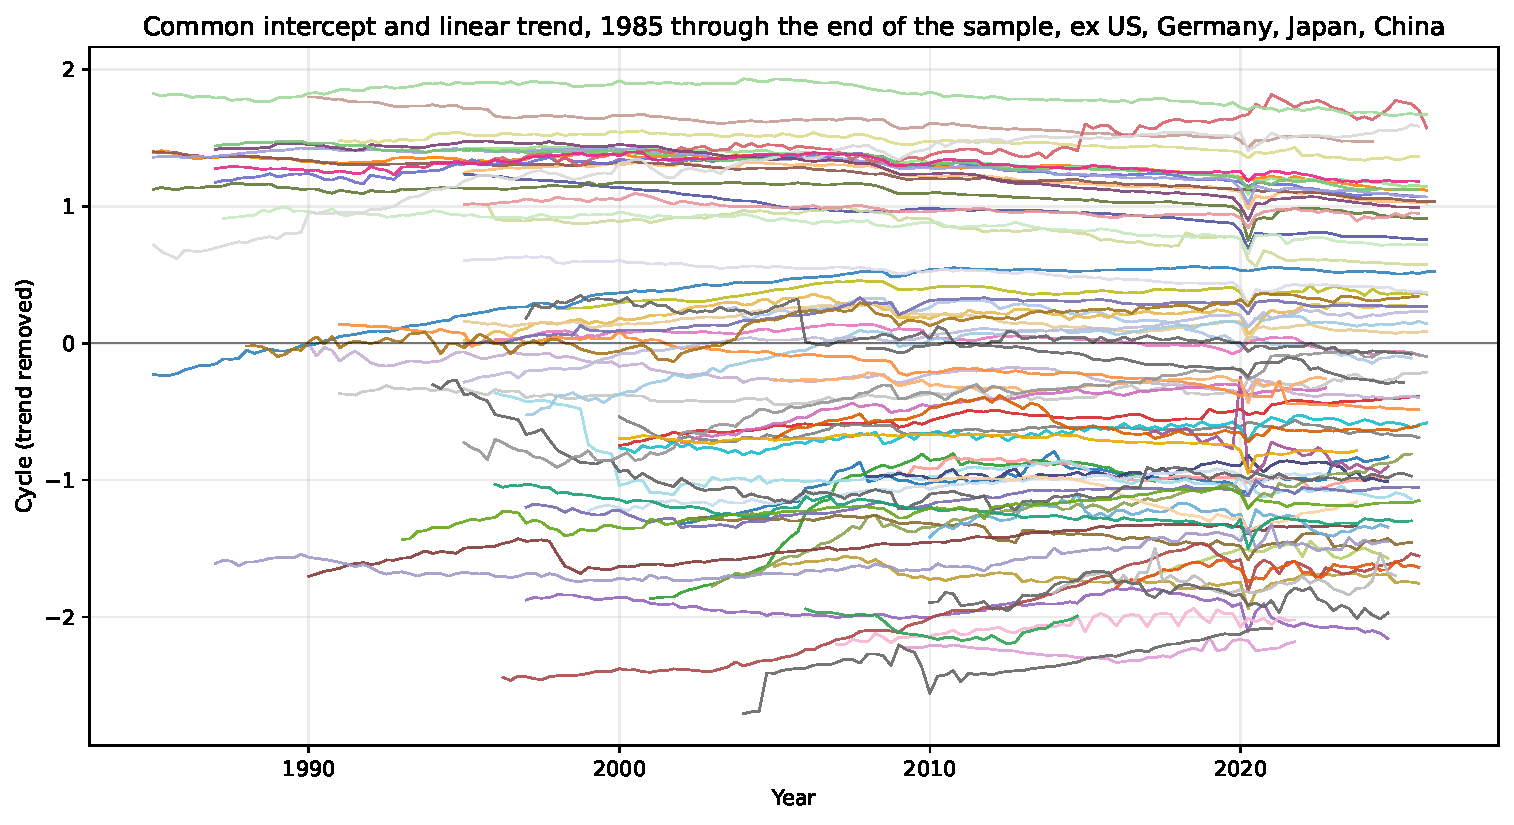
\includegraphics[width=0.75\textwidth]{figs/cycle_common_1985.pdf}
\caption{Country cycles $z_{it}=y_{it}-a-gt$.}
\end{figure}
\end{document}
